\chapter{Introducción}
\section{Problemática}

El presente proyecto aborda su problemática central a través de tres enfoques interrelacionados: primero, se destaca la importancia del control de calidad dentro de la industria de la moda; en segundo lugar, se identifican las ineficiencias inherentes al control de calidad tradicional; y finalmente, se subraya la creciente necesidad de automatización en el proceso de control de calidad.

\subsection*{Importancia del Control de Calidad en la Industria Textil}

Entre enero y mayo de 2022, las exportaciones de camisas, pantalones y camisetas en Perú experimentaron incrementos notables, con crecimientos del 57\%, 49\% y 31\% en valor, respectivamente. Hasta mayo de 2022, las exportaciones de confecciones alcanzaron los 759 millones de dólares americanos, marcando un aumento del 36\% en comparación con el año anterior \cite{LaCamara2022}. Estas estadísticas demuestran un crecimiento significativo en la exportación de prendas de vestir peruanas, por lo cual, es importante mantener altos estándares de calidad para satisfacer las expectativas de los mercados internacionales.

\begin{figure}[H]
	\centering
	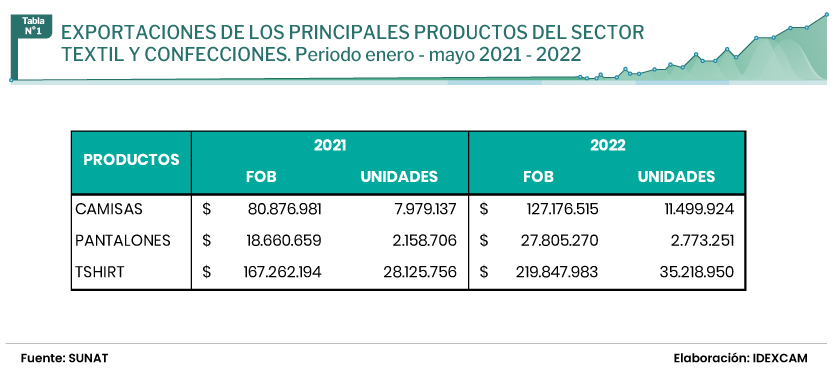
\includegraphics[width=0.8\textwidth]{img/exportaciones.jpg}
	\caption[Exportaciones peruanas de textiles: aumento en FOB y unidades, 2021 vs 2022.]{Exportaciones peruanas de textiles: aumento en FOB y unidades, 2021 vs 2022. Fuente \cite{LaCamara2022}.}
\end{figure}

El control de calidad en la industria textil es esencial para asegurar que las prendas no solo cumplan con los estándares de calidad establecidos, sino también que ofrezcan seguridad y durabilidad. Este proceso minucioso abarca diversas etapas, incluyendo la inspección de tejidos, la graduación de patrones, el corte, la costura, el acabado y finalmente, el empaquetado. Todo ello con el objetivo de garantizar que el producto final cumpla con las expectativas de los clientes. Entre los defectos más comunes que se identifican durante estas etapas se encuentran las variaciones de color, manchas, agujeros, puntadas rotas, costuras desalineadas, hilos sueltos, así como medidas incorrectas y tallas inconsistentes, tanto en los tejidos como en la construcción de las prendas \cite{TetraInspection2024}. 

\subsection*{Ineficiencias en el Control de Calidad Tradicional}

El enfoque tradicional de control de calidad, que se centra principalmente en inspecciones al final del proceso y en la implementación de correcciones a posterior, resulta en elevados costos debido a desechos y reparaciones. Este enfoque repercute negativamente en la competitividad y sostenibilidad de las empresas. Un estudio realizado por \cite{BonillaPastor2015} sobre la gestión de calidad en micro y pequeñas empresas (Mypes) del sector textil en Perú, destaca las graves consecuencias económicas y ambientales que surgen de una gestión de calidad ineficaz. Desde el punto de vista económico, los residuos y desperdicios producidos por procesos ineficientes constituyen un gasto promedio del 7.4\% en relación con el costo total de producción, lo cual impacta directamente en la competitividad y la rentabilidad de las empresas.

El control de calidad manual, como se observa en la Figura \ref{fig:insp_manual}, es ampliamente utilizada en procesos de producción debido a su relativa facilidad y la no necesidad de equipos técnicos especializados. Sin embargo, enfrenta desafíos significativos debido a factores humanos como los que se detallan en la Tabla \ref{tab:eficiencia_inspección}. Dichos factores inciden directamenteb en la efectividad del control de calidad manual, elevando potencialmente la incidencia de errores en la evaluación de la calidad. Investigaciones referenciadas en el estudio de \cite{KujawinskaVogt2015} revelan que, en tareas de inspección simples, la tasa de error puede fluctuar entre un 3\% y un 30\%, dependiendo de la índole de la tarea y las condiciones en que se efectúa la inspección.

\begin{figure}[H]
	\centering
	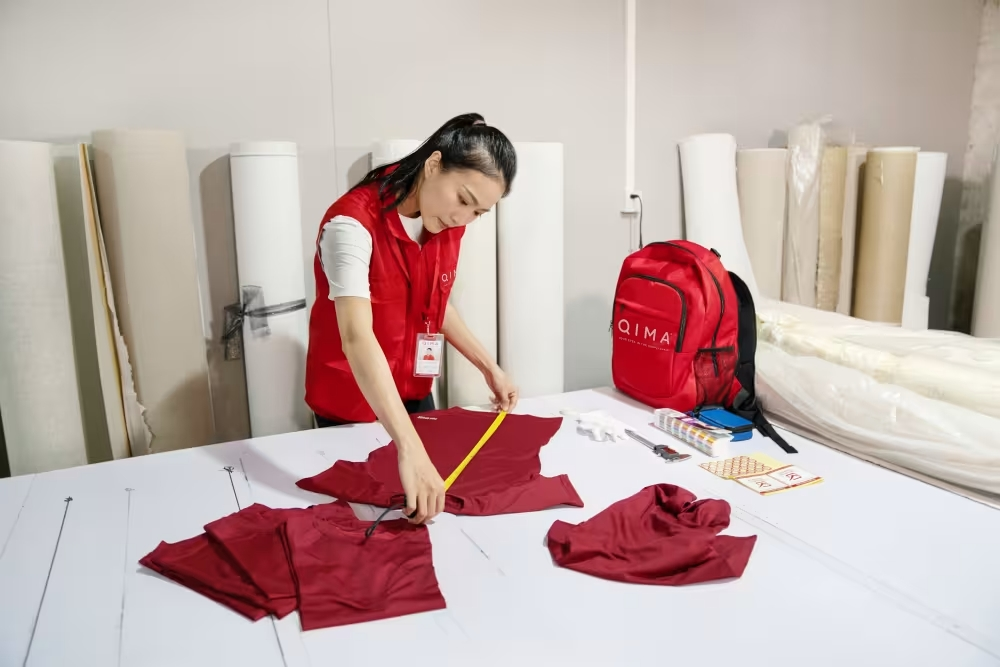
\includegraphics[width=0.65\textwidth]{img/insp_manual.jpg}
	\caption[Inspección manual de prendas de vestir.]{Inspección manual de prendas de vestir. Fuente: \cite{qimaProcedimientosInspeccin}.}
	\label{fig:insp_manual}
\end{figure}

\begin{table}[H]
	\centering
	\caption[Factores que afectan la eficiencia de la inspección visual.]{Factores que afectan la eficiencia de la inspección visual. Fuente: \cite{KujawinskaVogt2015}.}
	\begin{tabular}{|p{10em}|p{18em}|}
		\hline
		\textbf{Factors} & \textbf{Examples} \bigstrut\\
		\hline
		Technical & {Type of defects; Defect visibility; Quality level; Standards (tests); Control automation;  Other} \bigstrut\\
		\hline
		Psychophysical & Age;  Sex;  Observation  skills;  Experience;  Temperament;  Creativity;  Other \bigstrut\\
		\hline
		Organizational & Training;  Scope  of  decision  making; Feedback;  Precise  instructions;  Other \bigstrut\\
		\hline
		Workplace environment & {Light; Noise; Temperature; Work time; Workstation organization; Other} \bigstrut\\
		\hline
		Social & {Team communication;  Pressure;  Isolation; Other} \bigstrut\\
		\hline
	\end{tabular}%
	\label{tab:eficiencia_inspección}%
\end{table}%

\subsection*{Necesidad de Mejora y Automatización}

La integración de la Inteligencia Artificial (IA) en el control de calidad de la industria textil y de la moda ha introducido métodos avanzados para la inspección de calidad, desde la producción hasta la revisión final de las prendas. Esta innovación mejora significativamente la eficiencia y precisión, minimizando los errores humanos y los costos de producción, mientras asegura la adherencia a estándares de calidad elevados \cite{TextileLearner}. La Tabla \ref{tab:visual_vs_automated} resume la comparación entre inspección visual humana y la inspección automatizada. Estas limitaciones subrayan la necesidad de un proceso de inspección más automatizado y preciso para reducir errores y mejorar la eficiencia \cite{Islam2006ASuitable}.

\begin{table}[H]
	\centering
	\caption[Inspección visual versus inspección automatizada.]{Inspección visual versus inspección automatizada \cite{Islam2006ASuitable}.}
	\begin{tabular}{|p{13em}|c|c|}
		\hline
		\textbf{Inspection Type} & {\textbf{Visual}} & \textbf{Automated} \bigstrut\\
		\hline
		Fabric Types & 100\% & \multicolumn{1}{c|}{70\%} \bigstrut\\
		\hline
		Defect Detection Rate & 70\%  & 80\%+ \bigstrut\\
		\hline
		Reproducibility & 50\%  & 90\%+ \bigstrut\\
		\hline
		Objective Defect Judgment & 50\%  & {100\%} \bigstrut\\
		\hline
		Statistics Ability & 0\%   & 95\%+ \bigstrut\\
		\hline
		Inspection Speed & {30 m/min} & {120 m/min} \bigstrut\\
		\hline
		Response Type & 50\%  & {80\%} \bigstrut\\
		\hline
		Information Content & 50\%  & 90\%+ \bigstrut\\
		\hline
		Information Exchange & 20\%  & 90\%+ \bigstrut\\
		\hline
	\end{tabular}%
	\label{tab:visual_vs_automated}%
\end{table}%

La automatización en la detección de defectos mediante visión artificial es crucial en manufactura, mejorando la consistencia y reduciendo errores humanos. La inspección óptica automatizada, impulsada por aprendizaje profundo y machine learning, supera los métodos manuales, ofreciendo eficiencia y precisión. Esto facilita la identificación rápida y confiable de defectos, elevando la calidad del producto y disminuyendo costos y tiempos de producción. La utilización de redes neuronales convolucionales para la extracción de características mejora la adaptabilidad y eficiencia de la inspección, siendo clave para el avance en manufactura. \cite{SanchezRomero2023}.

\section{Propuesta de Solución}

\section{Objetivos}

El proyecto presenta un objetivo general del cual surgen \ref{lst:objetivos_especificos} objetivos específicos para lograr el cumplimiento del objetivo general.

\subsection{Objetivo General}

Desarrollar un sistema integrado para el control de calidad de prendas de vestir, que combine tecnologías de visión artificial y detección de metales para inspeccionar cada prenda de manera individual, asegurando su conformidad con los estándares de calidad establecidos en la ficha técnica de la prenda, tales como la ausencia de defectos visibles, la precisión en las medidas de talla y la detección de elementos metálicos extraños.

\subsection{Objetivos Específicos}

\begin{enumerate}
	\setlength\itemsep{-0.5em}
	\item Realizar una revisión bibliográfica (estado del arte) que permita definir los requerimientos del diseño del sistema y todo lo concerniente al diseño conceptual.
	
	\item Definir las exigencias específicas que debe cumplir el sistema para lograr el objetivo principal.
	
	\item Seguir la metodología de diseño basada en la norma VDI 2206 para el diseño mecatrónico completo del sistema.
	
	\item Diseñar un subsistema mecánico que permita transportar las prendas de vestir a través de los distintos módulos del sistema.
	
	\item Diseñar un subsistema de inspección por procesamiento de imágenes para realizar la medición de la talla de las prendas y realizar la verificación según la ficha técnica de la prenda.
	
	\item Diseñar un subsistema de detección de metales que examine cada prenda para identificar y alertar sobre la presencia de agujas, alfileres o cualquier otro elemento metálico extraño, garantizando así la seguridad del producto final.
	
	\item Desarrollar una interfaz intuitiva para mostrar resultados de detección de calidad de prendas, incluyendo visualización de defectos, mediciones de tallas e identificación de metales
	
	\item Seleccionar el concepto de solución óptimo basados en los criterios técnicos y económicos, según la norma VDI 2225.
	
	\item Estimar un costo de fabricación de un prototipo a partir de los componentes seleccionados.
	
	\label{lst:objetivos_especificos}
\end{enumerate}

\section{Metodología}
% BENDEZU_LEDESMA_JORGE_DISEÑO_PROTOTIPO_DRON

Para el desarrollo del presente trabajo se emplearan adaptaciones de las metodologías diseñadas por la VDI (Asociación Alemana de Ingenieros). Entre ellas, se utilizar una adaptación de la metodología VDI 2206 \cite{VDIVDE2206_2021} y de la metodología VDI 2221 \cite{VDI2221_2019} para el diseño conceptual, el cual consistirá en las siguientes etapas: Elaboración de lista de requerimientos, Elaboración de un diagrama de funciones y Elaboración de una matriz morfológica (con 3 soluciones). Posteriormente se seguirá una adaptación de la metodología VDI 2225 \cite{VDI2225_series} para realizar un análisis técnico y económica de las soluciones.

De ese modo, los Capítulos 1 y 2 se enfocaran en a comprender la problemática de la investigación. El Capítulo 1 aborda una investigación preliminar para contextualizar el problema, identificar los enfoques de la problemática y definir el alcance de la solución. El Capítulo 2, por su parte, examina el estado actual de la tecnología para establecer un marco de referencia que permita evaluar la viabilidad del proyecto, con el fin de determinar parámetros y características relevantes para el sistema de control de calidad en prendas de vestir.

En el Capítulo 3, se desarrollan los procesos de la metodología correspondientes para diseñar la estructura de funciones y el concepto de solución. Utilizando la lista de requerimientos, se abstrae el problema para obtener una comprensión amplia de las funciones necesarias, lo que guía el diseño mecánico y eléctrico inicial y ayuda a determinar los sensores, actuadores y fuentes de energía necesarios. A partir de esta estructura, se crea una matriz morfológica que facilita la combinación de distintas alternativas de solución, culminando en la definición precisa de los objetivos de diseño e implementación. Además, se realizará una ponderación de los conceptos de solución a través de un análisis técnico-económico con el objetivo de obtener un concepto de solución óptimo.

Por último, en los capítulos subsecuentes se realizaran los siguientes partes del trabajo:

\begin{itemize}
	\setlength\itemsep{-0.5em}
	\item Realización de cálculos mecánicos, electrónicos y de control necesarios para determinar las características de la máquina.
	\item Se va a seleccionar (o diseñar) un modelo de inteligencia artificial para realizar la labor de la visión artificial del sistema, además, se va a buscar, o en su defecto, se va a crear un dataset para entrenar un modelo de inteligencia artificial.
	\item Verificación de las partes mecánicas por medio de software de elementos finitos.
	\item Elaboración de planos y estimación de costos de fabricación.
\end{itemize}

\section{Alcance de la Investigación}

Este trabajo se enfoca en el diseño de un sistema a través del dimensionamiento detallado de cada uno de sus componentes. El objetivo principal es lograr que el sistema opere de manera autónoma. En otras palabras, se busca reducir la intervención humana al mínimo necesario. Esta intervención se limita a tareas como la inserción de la prenda a verificar en el sistema, el ingreso de señales de control y la posterior retirada de la prenda ya evaluada. Es importante destacar que los requisitos definidos para este proyecto, desarrollados a lo largo de la investigación, están orientados a un entorno no industrial. Además, se señala que el prototipo busca alcanzar un Nivel 4 de Madurez Tecnológica (TRL4), mediante simulaciones que se llevarán a cabo tanto en software como a través de un Producto Mínimo Viable (MVP) en un entorno de laboratorio controlado.

Para concluir, esta tesis presentará todos los cálculos de diseño necesarios, así como los planos mecánicos y electrónicos, los materiales escogidos para el proyecto, y los diagramas de flujo que explican la operación y control del sistema.